\section{Appendices}\label{sec:app:app}

\textbf{Appendix A:}

The FPGA on MP7 board receives and transmits data via GTH transceivers.\\
In Figure~\ref{fig:app:gth_conf} configuration of GTHs~\cite{GTHs} for Global Trigger is shown.

\begin{figure}[htb]
\centering
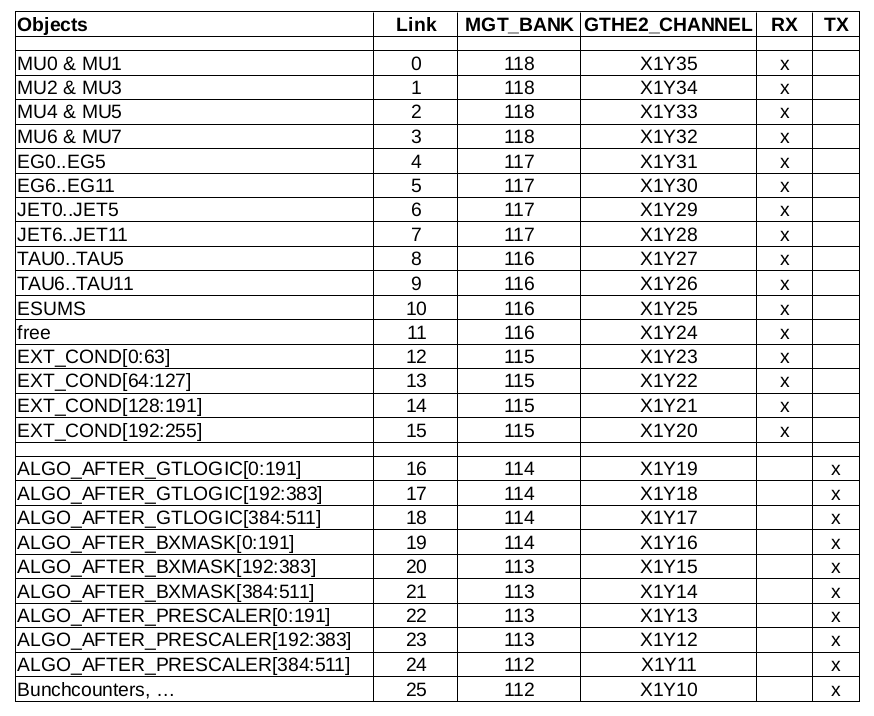
\includegraphics[width=15cm]{figures/gth_xc7v690t_ffg1927}
\caption{Configuration of GTHs}
\label{fig:app:gth_conf}
\end{figure}

\clearpage

\textbf{Appendix B:}

Figure~\ref{fig:app:ugt_inputs} shows the configuration of optical links to Global Trigger.\\
Links 0..3 contains muon data from GMT, links 4..11 data from GCT and links 12..15 external conditions
from AMC502 boards.

\begin{figure}[htb]
\centering
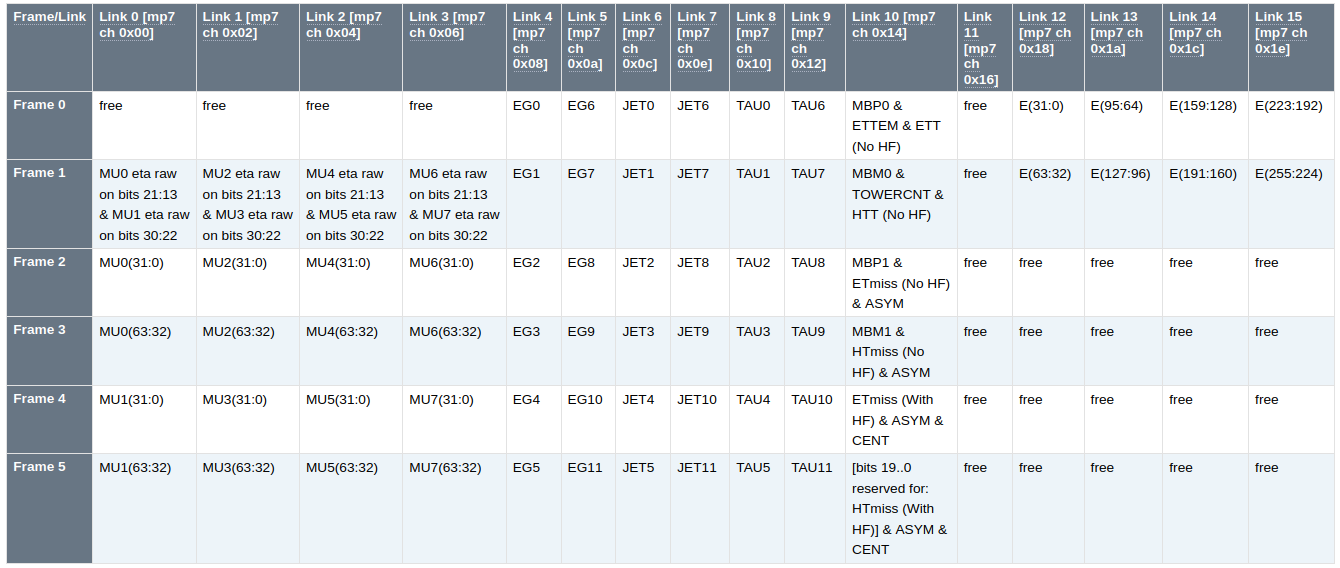
\includegraphics[width=15cm]{figures/ugt_inputs}
\caption{Optical link inputs to Global Trigger}
\label{fig:app:ugt_inputs}
\end{figure}

\textbf{Appendix C:}

Figure~\ref{fig:app:ugt_outputs} shows the configuration of links from Global Trigger to AMC13 (readout).\\
Links 16..24 contains algo data (after GTL, after BX mask and after prescalers), link 25 contains several counter values.

\begin{figure}[htb]
\centering
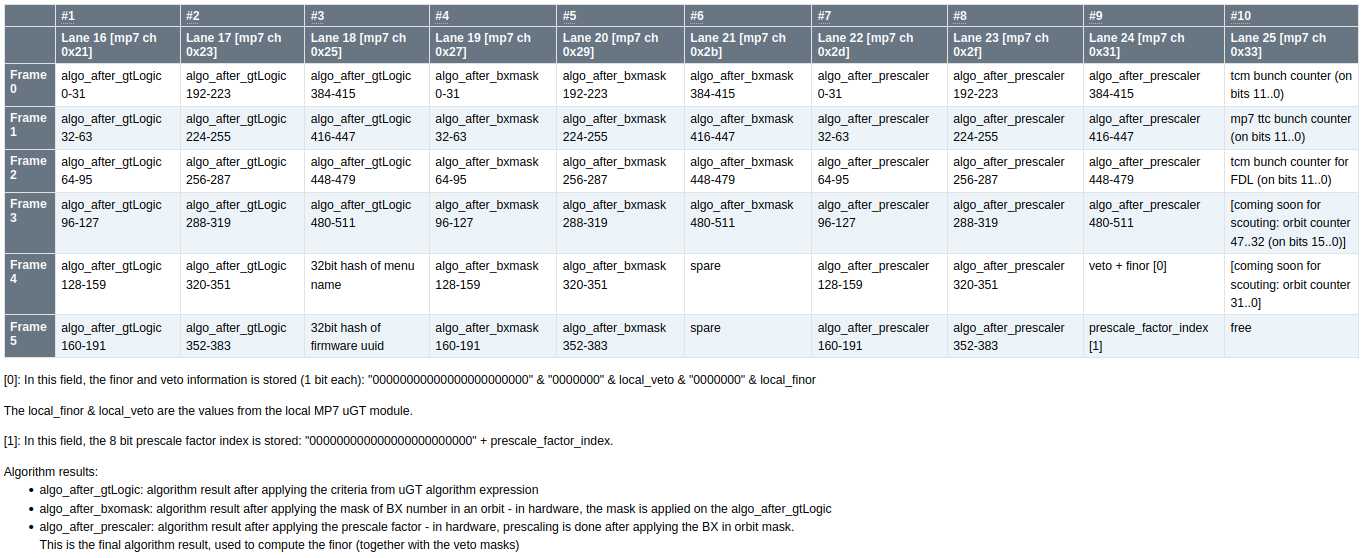
\includegraphics[width=15cm]{figures/ugt_outputs}
\caption{Outputs from Global Trigger to AMC13}
\label{fig:app:ugt_outputs}
\end{figure}

\clearpage

\textbf{Appendix D:}

Figure~\ref{fig:app:ugt_pp} shows the connections on Global Trigger patch panel for optical links.

\begin{figure}[htb]
\centering
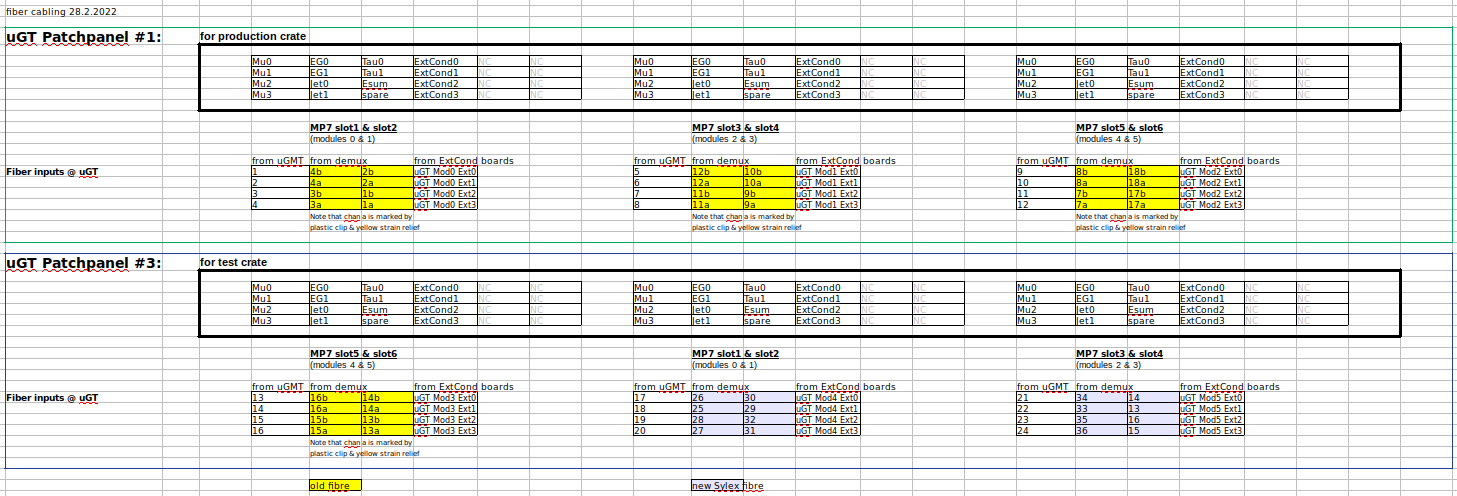
\includegraphics[width=15cm]{figures/ugt_patchpanel}
\caption{Global Trigger patch panel for optical link}
\label{fig:app:ugt_pp}
\end{figure}

\clearpage
